

%%%% EVENT1
\FullBackgroundPicture{../montecarlo/figures/event1}
\begin{frame}\frametitle{Modelling of hadron collisions}
\small\centering

\begin{flushright}\tiny Drawings from~\cite{Gieseke}\end{flushright}

want to do physics at hadron colliders?

need a good understanding of incoming hadrons

\myskip
\myskip

%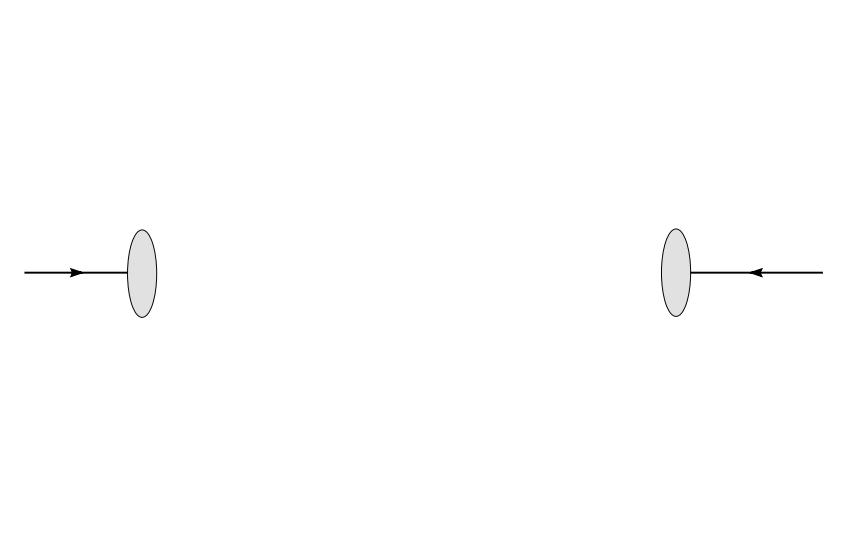
\includegraphics[height=0.8\textheight]{../montecarlo/figures/event1}

$E(p_1)=4\tev$ \hspace{.3\paperwidth} $E(p_2)=4\tev$

\vspace{.3\paperheight}

Quarks are distributed according to PDFs inside the proton\\
{\LARGE $\Downarrow$}\\
intial energy unknown, $P($valence quarks$)\sim \frac{1}{2}P(p)$

\end{frame}


%%%% EVENT1
\FullBackgroundPicture{../montecarlo/figures/event2}
\begin{frame}\frametitle{Hard scattering of two partons}
\centering\myskip
%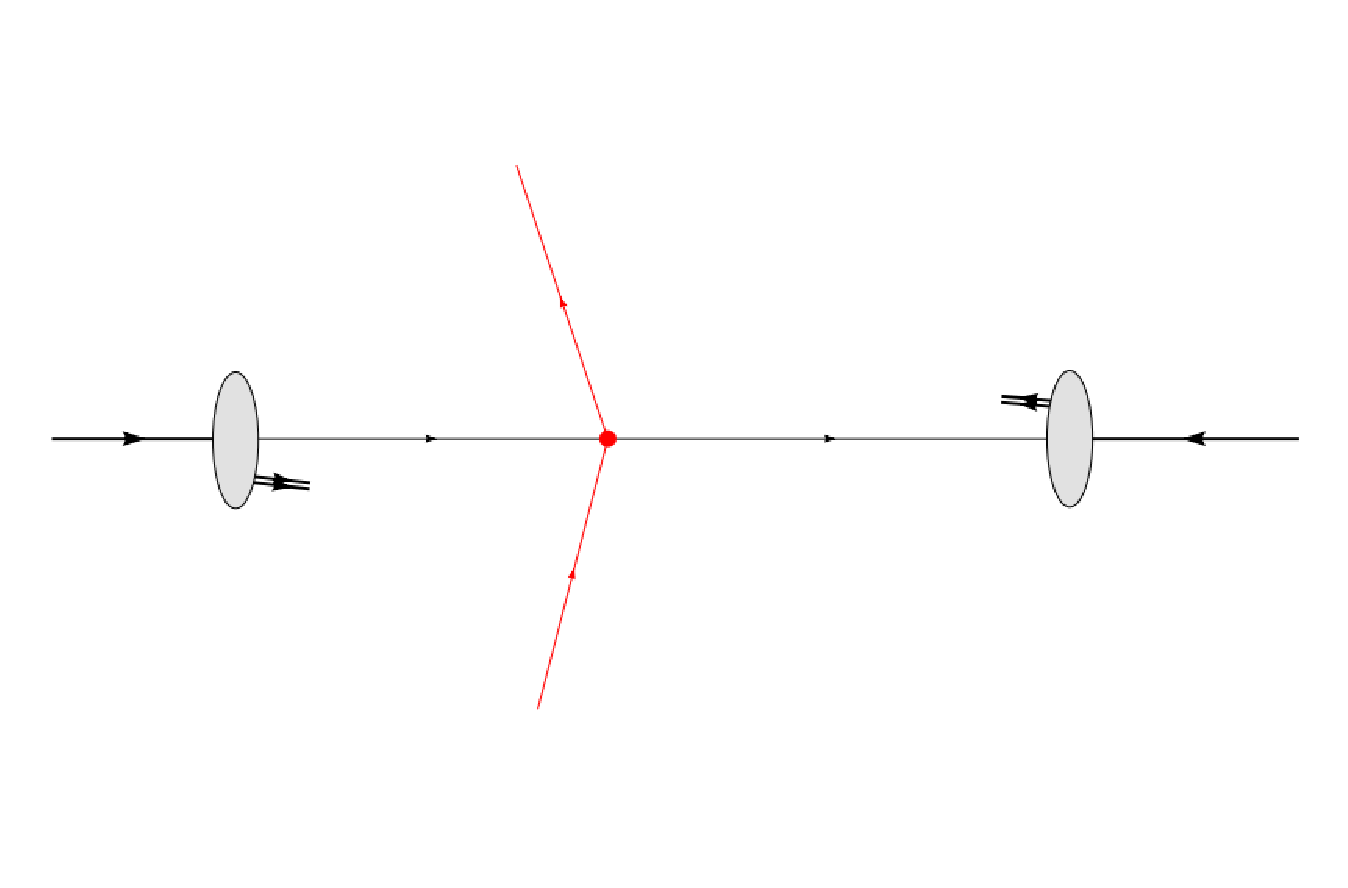
\includegraphics[height=0.8\textheight]{../montecarlo/figures/event2}

\begin{minipage}{.25\textwidth}\centering
$\quad$
\end{minipage}\begin{minipage}{.7\textwidth}\centering
\begin{flushright}\footnotesize {\it MC: Matrix Element computation\\\myskip LO (\texttt{ALPGEN}) and NLO (\texttt{MC@NLO,POWHEG}) generators}
\end{flushright}
\end{minipage}


\vspace{.42\paperheight}

{\cccolor asymptotic freedom}: high energy $\longleftrightarrow$ low \alphas\\
{\LARGE $\Downarrow$}\\
(fixed order) pQCD

\begin{flushright}\scriptsize Thanks {\cccolor factorization theorem}!
\end{flushright}

\end{frame}

%%%% EVENT1
\FullBackgroundPicture{../montecarlo/figures/event4}
\begin{frame}\frametitle{Parton showering}
\centering\myskip


\begin{minipage}{.5\textwidth}\centering
$\quad$
\end{minipage}\begin{minipage}{.45\textwidth}\centering
\begin{flushright}\footnotesize {\it MC: iterative evolution different for\\Final- and Initial-state radiation\\\myskip (\texttt{PYTHIA,HERWIG})}\end{flushright}
\begin{flushright}\footnotesize {\it ME and PS matching}\end{flushright}
\end{minipage}

\vspace{.35\paperheight}

%real radiative corrections to any inclusive quantity

QCD emission: $q\to gq$, $g\to gg$, $g\to q\bar{q}$\\
{\LARGE $\Downarrow$}\\
higher-order corrections 


\end{frame}

%%%% EVENT1
\FullBackgroundPicture{../montecarlo/figures/event6}
\begin{frame}\frametitle{Hadronization}
\centering


\begin{minipage}{.25\textwidth}\centering
$\quad$
\end{minipage}\begin{minipage}{.7\textwidth}\centering
\begin{flushright}
\vskip-5ex

\footnotesize {\it MC: phenomenological models}\\
\includegraphics[width=.6\textwidth,height=.35\textheight]{pics/hadronization.jpg}\\
{\scriptsize\it color connections,\\ Lund string and cluster models\\(\texttt{PYTHIA,HERWIG})}
\end{flushright}
\end{minipage}

\vspace{.25\paperheight}

{\cccolor confinement} @ $Q\sim 1\gev$\\
{\LARGE $\Downarrow$}\\
free partons cannot exist


\end{frame}


%%%% EVENT1
%\FullBackgroundPicture{../montecarlo/figures/event7}
\FullBackgroundPicture{../montecarlo/figures/my_collision}
\begin{frame}\frametitle{Underlying event simulation}
\centering
%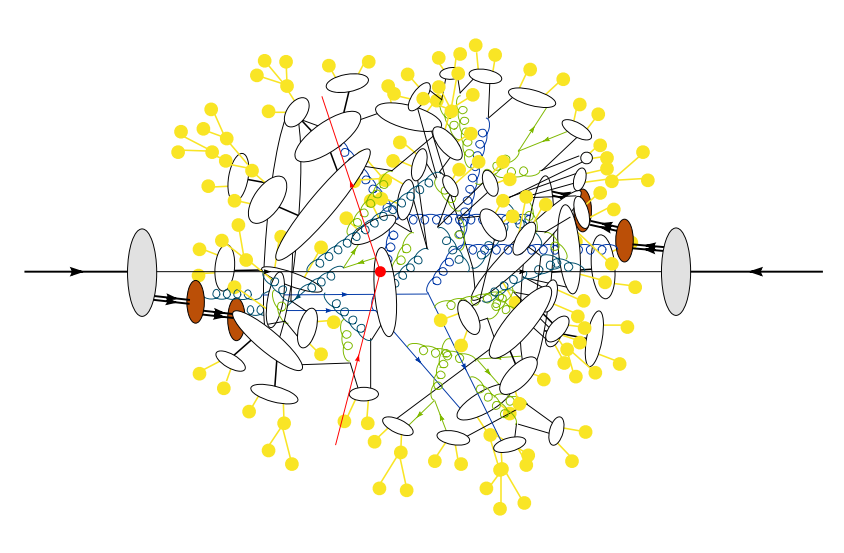
\includegraphics[height=0.8\textheight]{../montecarlo/figures/event7}


\begin{minipage}{.65\textwidth}\centering
$\quad$
\end{minipage}\begin{minipage}{.35\textwidth}\centering\footnotesize
hadron remnants\\ interact too\\
{\LARGE $\Downarrow$}\\
{\it phenomenological\\ models tuned on\\
``low-\pt'' events}
\end{minipage}

\vspace{.5\paperheight}


\end{frame}


\BackgroundPicture{pics/emptyIMG}
\begin{frame}\frametitle{Pile-up}
\centering\myskip

\begin{minipage}{.35\textwidth}\centering
\footnotesize

But \sout{problems} collisions\\
never come alone\dots

\begin{itemize}
\item {\cccolor in-time} and {\cccolor out-of-time} pile-up events
\end{itemize}

\myskip
high $\mathcal{L}$\\
{\LARGE $\Downarrow$}\\

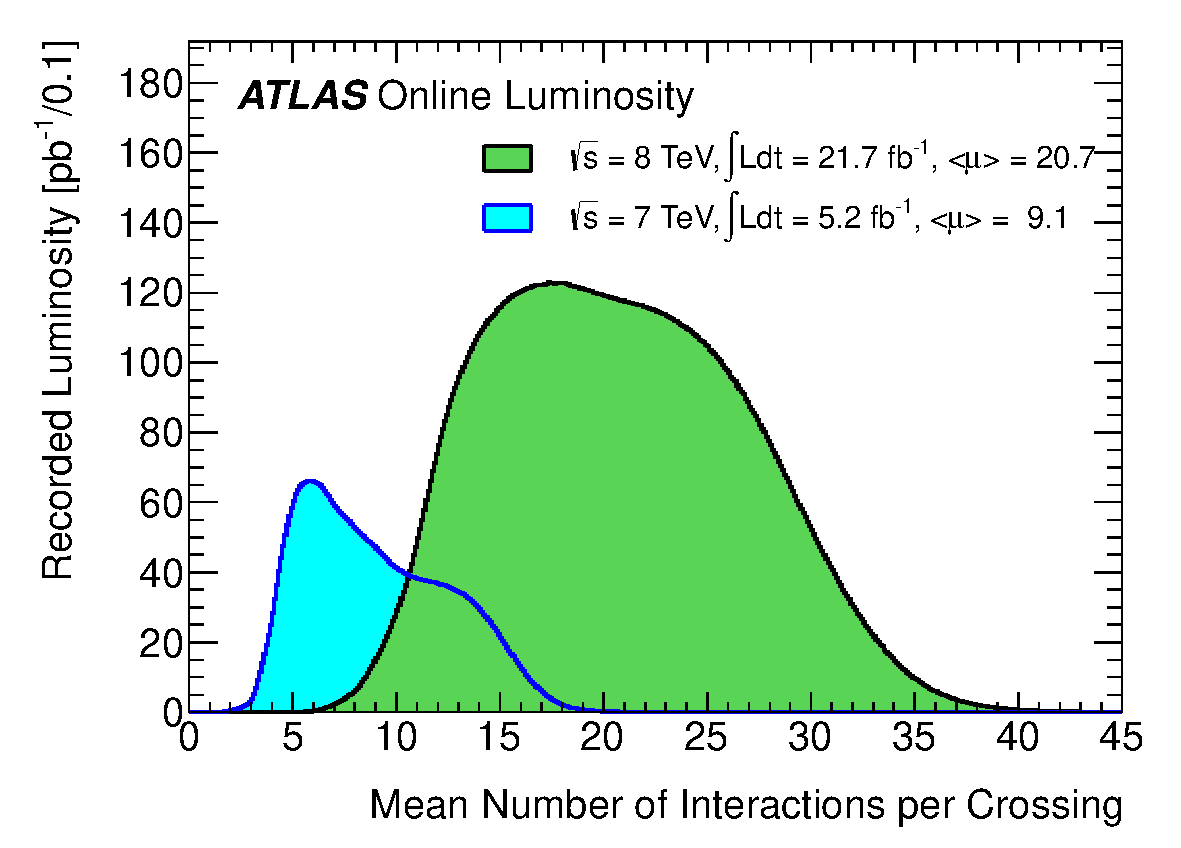
\includegraphics[width=1.\textwidth]{pics/mu_2011_2012-dec.pdf}



\end{minipage}\begin{minipage}{.65\textwidth}\centering

\vskip-5ex
\footnotesize
real $Z\to\mu\mu$ event with high pile-up (25 vertices)

\includegraphics[height=0.9\textheight,width=1.\textwidth]{pics/2012_highPileup.png}

\tiny
from \url{https://twiki.cern.ch/twiki/bin/view/AtlasPublic/EventDisplayStandAlone}
\end{minipage}

\end{frame}
